\documentclass[a4paper,11pt]{ujreport}
%%【PostScript, JPEG, PNG等の画像の貼り込み】
%% 利用するパッケージを選んでコメントアウトしてください.
\usepackage{graphicx} % for 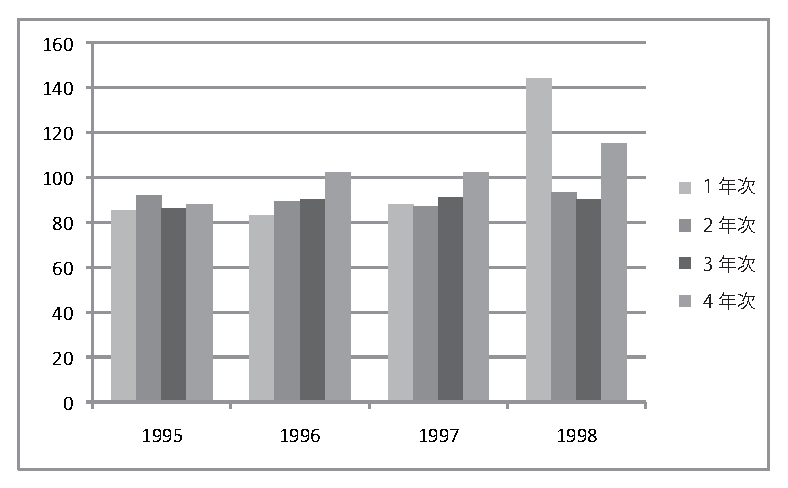
\includegraphics[width=3cm]{sample.eps}
\usepackage{epsfig} % for 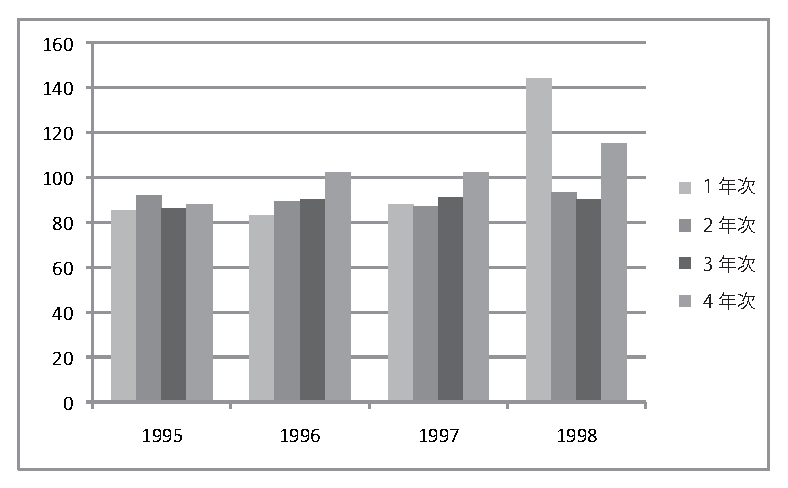
\psfig{file=sample.eps,width=3cm}
%\usepackage{epsf} % for \epsfile{file=sample.eps,scale=0.6}
%\usepackage{epsbox} % for \epsfile{file=sample.eps,scale=0.6}
\usepackage{/Users/takagihayata/workspace/materialize-mongodb/paper/mast/class/mediabb} % for pdf

\usepackage{times} % use Times Font instead of Computer Modern
% \usepackage{listings} % for soursecode
% \usepackage{plistings} % for soursecode
\usepackage{/Users/takagihayata/workspace/materialize-mongodb/paper/mast/class/docmute} % texファイル分割用

\setcounter{tocdepth}{3}
\setcounter{page}{-1}

\setlength{\oddsidemargin}{0.1in}
\setlength{\evensidemargin}{0.1in}
\setlength{\topmargin}{0in}
\setlength{\textwidth}{6in}
%\setlength{\textheight}{10.1in}
\setlength{\parskip}{0em}
\setlength{\topsep}{0em}

%\newcommand{\zu}[1]{{\gt \bf 図\ref{#1}}}

%% タイトル生成用パッケージ(重要)
\usepackage{/Users/takagihayata/workspace/materialize-mongodb/paper/mast/class/mast-jp-sjis}

%% タイトル
%% 【注意】タイトルの最後に\\ を入れるとエラーになります
\title{NoSQL型データベースシステムでの実体化ビュー選択に関する研究}
%% 著者
\author{髙木 颯汰}
%% 指導教員
\advisor{古瀬 一隆 陳 漢雄}

%% 年月 (提出年月)
%% 年月は必要に応じて書き替えてください.
\majorfield{ } \yearandmonth{2019年 1月}


\addtocounter{page}{2} %単体でコンパイルした際の調整用
\addtocounter{chapter}{3} %単体でコンパイルした際の調整用
\begin{document}

\chapter{実験}
\label{chap:Experiment}
\section{Mongooseについて}
MongooseとはMongoDB用モデリングツールで,Node.jsの非同期環境でうまく動作することを目的として設計されている.Mongooseを使用すれば,モデルを定義して操作することで,MongoDBのコレクション/ドキュメントを操作できる\cite{mongoose}.本論文ではMongooseを用いてMongoDBを操作するミドルウェアを実装する.

\section{実験環境}
実験環境に関する情報を表\ref{table:experiment_env}に示す.
\begin{table}[htb]
  \begin{center}
    \caption{実験環境}
		\label{table:experiment_env}
    \begin{tabular}{|c|c|} \hline
      マシン & MacBook (Retina, 12-inch, 2017) \\ \hline
      プロセッサ & 1.2 GHz Intel Core m3\\ \hline
      メモリ & 8 GB 1867 MHz LPDDR3\\ \hline
      データベースシステム & Mongodb version 3.1.10\\ \hline
    \end{tabular}
  \end{center}
\end{table}

\section{実験方法}
本論文の実験で用いたコレクションは本のレビューサイトのデータベースを想定し作成した.personコレクション,storyコレクション,commentコレクション,publisherコレクションがある.コレクションの構造,コレクション同士の参照に関しては図\ref{figure:ExperimentCollection},図\ref{figure:ExperimentCollection2}に示す.storyコレクションには筆者として1つのpersonドキュメントのidを格納する.このstoryドキュメントが検索された際には筆者のidをperosnコレクションから検索し,結合して結果を返す.同じようにファンとしてpersonドキュメントのidを配列で格納することで複数のpersonドキュメントをstoryドキュメントに埋め込む.実際の実験データではファンとして1から100のpersonドキュメントのidを埋め込む.出版社としてpublisherドキュメントのidも格納する.

コレクションの特性として,storyドキュメントに数十のドキュメントが参照されているので,参照型のデータモデルでは結合処理が多く発生する.逆に埋込型のデータモデルではpersonドキュメントの更新の際に埋込先のstoryドキュメントの更新処理が増加する.

\begin{figure}[htbp]
	\begin{center}
		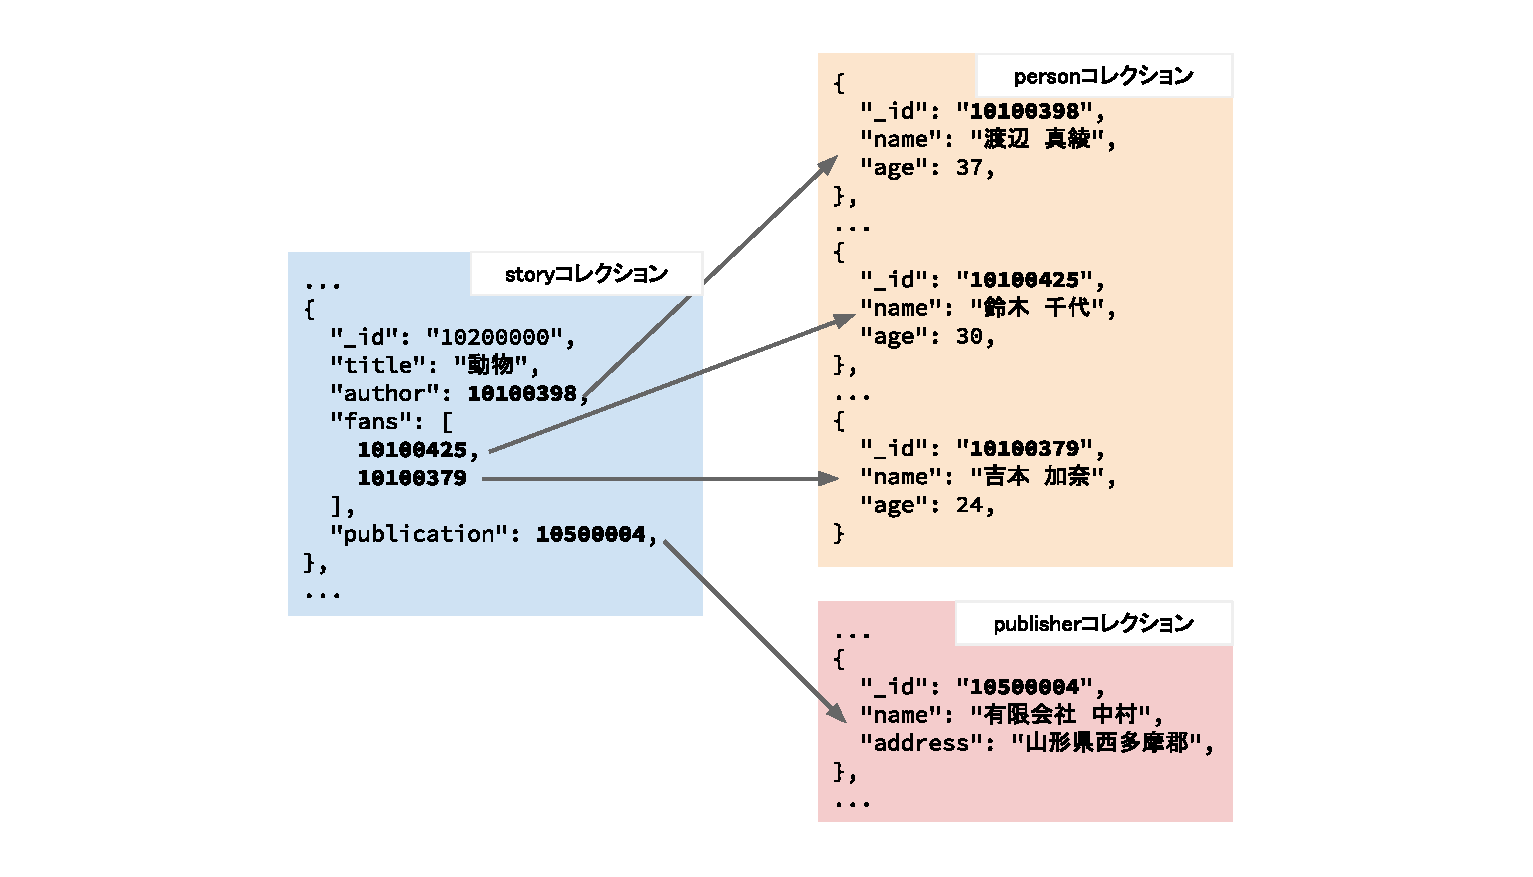
\includegraphics[width=30em, trim=10em 2em 10em 0]{src/ExperimentCollection.eps} %[trim=left bottom right top]
	\end{center}
	\caption{storyコレクションから各コレクションへの参照}
	\label{figure:ExperimentCollection}
\end{figure}
\begin{figure}[htbp]
	\begin{center}
		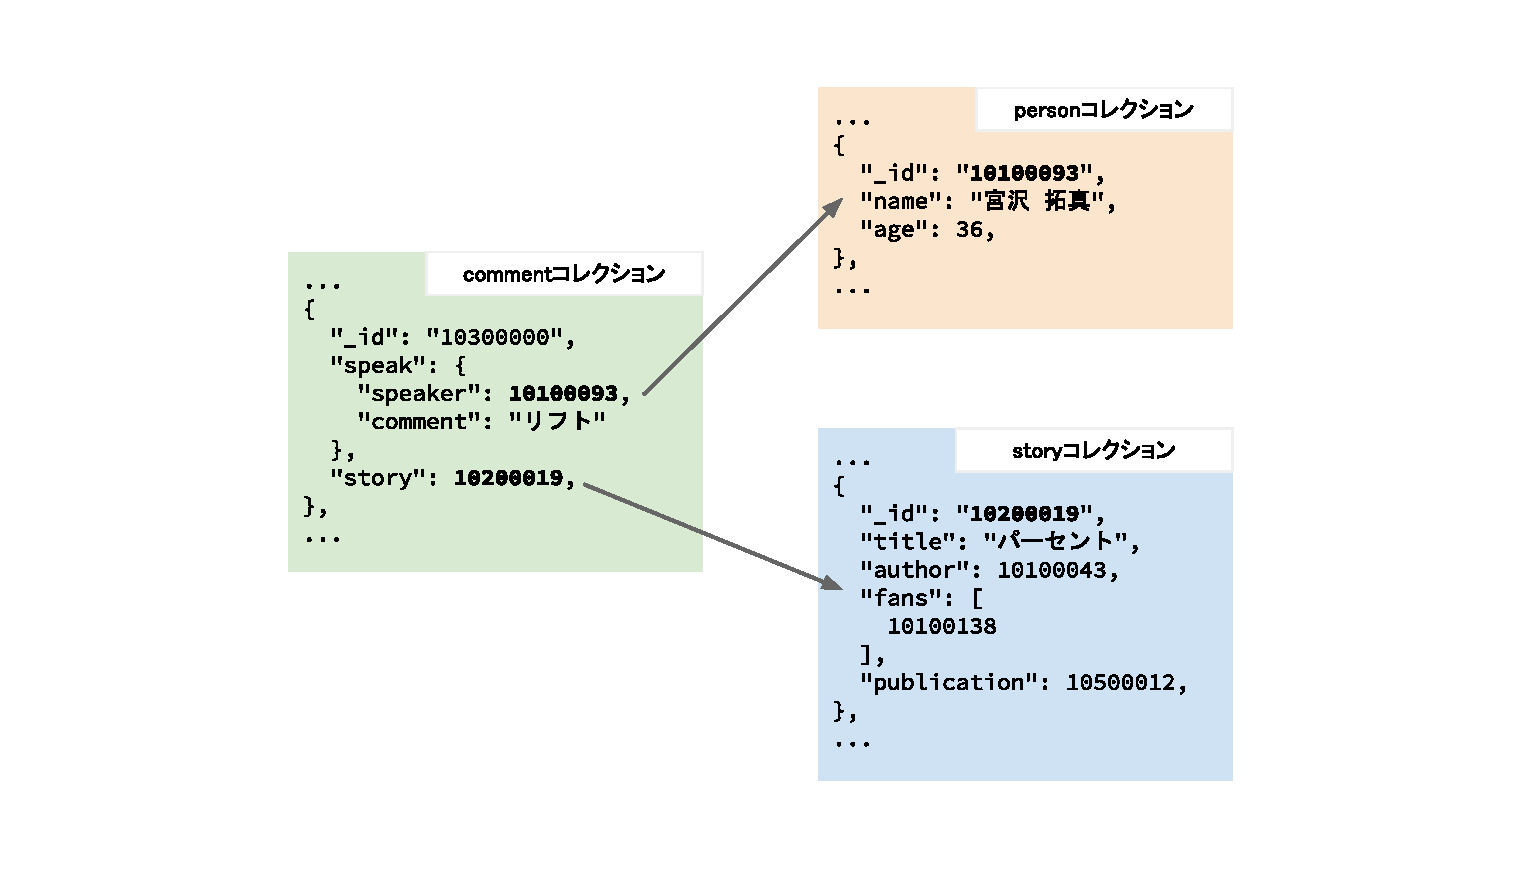
\includegraphics[width=30em, trim=10em 2em 10em 2em]{src/ExperimentCollection2.eps} %[trim=left bottom right top]
	\end{center}
	\caption{commentコレクションから各コレクションへの参照}
	\label{figure:ExperimentCollection2}
\end{figure}
実験において使用するデータは全て参照型のデータモデルで挿入する.実体化していない状態で検索された場合には結合処理を行い結果を返す.実験に用いるドキュメントはPythonのライブラリであるfaker\cite{faker}を用いて作成した.各コレクションに対して1000ドキュメントを作成した.


実験では全てのコレクションが従来の参照型のデータモデルを用いたシステムと実体化条件を用いずに全てのコレクションを実体化したシステム,実体化条件を用いて適宜コレクションを実体化するシステムの3つのデータベースシステムを比較する.その際,実体化を用いたシステムでは検索や更新を提案ミドルウェアを用いて処理する.

この3つのシステムを比較する際,検索と更新の比率を変えた5つのクエリパターンを用いて行う.このクエリパターンを表に示す.このパターンを用いて実験A,B,C,D,Eを行う.
\begin{table}[htb]
  \begin{center}
    \caption{クエリパターン}
		\label{table:experiment_query_pattern}
    \begin{tabular}{|c|c|c|} \hline
        & 検索回数比 & 更新回数比 \\ \hline
      パターンA & 99.9 & 0.1\\ \hline
      パターンB & 99 & 1\\ \hline
      パターンC & 97 & 3\\ \hline
			パターンD & 95 & 5\\ \hline
      パターンE & 90 & 10\\ \hline
    \end{tabular}
  \end{center}
\end{table}
それぞれのパターンに対して,使用したクエリを表\ref{table:ExperimentFindQuery}と表\ref{table:ExperimentUpdateQuery}で示す.MongoDBのドライバのみを用いる場合には\ref{section:AboutMvInDocumentDB}節で説明した様に集計機能を用いて結合処理を実現したが,Mongooseではpopulateメソッドでアプリケーションレベルでの結合処理を実現しており,内部的にはfindメソッドを複数に分けて実行し,アプリケーション側で結合処理を行う.表\ref{table:ExperimentFindQuery}のクエリはMongooseのpopulateメソッドを用いて結合処理をおこなっており,commentコレクションのクエリを例とすると,idがTestIDのcommentドキュメントを"speak.speaker"と"story"のフィールドを結合した状態でfindする処理である.内部的にはcomment,person,storyコレクションに対してクエリを発行している.

提案手法を用いる場合には検索・更新に関わらずクエリが数回処理された際に実体化条件を検討し,適宜実体化ビューを作成,破棄を行う.

\begin{table}[htb]
  \begin{center}
    \caption{実験で使用した検索クエリ}
		\label{table:ExperimentFindQuery}
    \begin{tabular}{|c|l|} \hline
      コレクション & \multicolumn{1}{|c|}{クエリ}\\ \hline
      person &
      \begin{tabular}{l}
        db.person.find(\{\_id: testID\})\\
        \ \ .populate([]);
      \end{tabular}\\ \hline
			story &
      \begin{tabular}{l}
        db.story.find(\{\_id: testID\})\\
        \ \ .populate(["author", "fans", "publication", "comments"]);
      \end{tabular}\\ \hline
      comment &
      \begin{tabular}{l}
        db.comment.find(\{\_id: testID\})\\
        \ \ .populate(["speak.speaker", "story"]);
      \end{tabular}\\ \hline
      publisher &
      \begin{tabular}{l}
        db.publisher.find(\{\_id: testID\})\\
        \ \ .populate([]);
      \end{tabular}\\ \hline
    \end{tabular}
  \end{center}
\end{table}
\begin{table}[htb]
  \begin{center}
    \caption{実験で使用した更新クエリ}
		\label{table:ExperimentUpdateQuery}
    \begin{tabular}{|c|l|} \hline
      コレクション & \multicolumn{1}{|c|}{クエリ}\\ \hline
      person &
      \begin{tabular}{l}
        db.person.update(\\
        \ \ \{\_id: testID\},\\
        \ \ \{\$set: \{name: "太郎"\}\\
        \});
      \end{tabular}\\ \hline
			story &
      \begin{tabular}{l}
        db.story.update(\\
        \ \ \{\_id: testID\},\\
        \ \ \{\$set: \{title: "研修資料"\}\\
        \});
      \end{tabular}\\ \hline
      comment &
      \begin{tabular}{l}
        db.comment.update(\\
        \ \ \{\_id: testID\},\\
        \ \ \{\$set: \{"speak.comment": "いい天気"\}\\
        \});
      \end{tabular}\\ \hline
      publisher &
      \begin{tabular}{l}
        db.publisher.update(\\
        \ \ \{\_id: testID\},\\
        \ \ \{\$set: \{address: "つくば市天王台"\}\\
        \});
      \end{tabular}\\ \hline
    \end{tabular}
  \end{center}
\end{table}

\end{document}
